%%%%%%%%%%%%%%%%%%%%%%%%%%%%%%%%%%%%%%%%%
% Structured General Purpose Assignment
% LaTeX Template
%
% This template has been downloaded from:
% http://www.latextemplates.com
%
% Original author:
% Ted Pavlic (http://www.tedpavlic.com)
%
% Note:
% The \lipsum[#] commands throughout this template generate dummy text
% to fill the template out. These commands should all be removed when 
% writing assignment content.
%
%%%%%%%%%%%%%%%%%%%%%%%%%%%%%%%%%%%%%%%%%

\documentclass{article}

\usepackage{fancyhdr} % Required for custom headers
\usepackage{lastpage} % Required to determine the last page for the footer
\usepackage{extramarks} % Required for headers and footers
\usepackage{graphicx} % Required to insert images
\usepackage[utf8]{inputenc}

% Margins
\topmargin=-0.45in
\evensidemargin=0in
\oddsidemargin=0in
\textwidth=6.5in
\textheight=9.0in
\headsep=0.25in 

\linespread{1.1} % Line spacing



\setlength\parindent{0pt} % Removes all indentation from paragraphs

%----------------------------------------------------------------------------------------
%	DOCUMENT STRUCTURE COMMANDS
%	Skip this unless you know what you're doing
%----------------------------------------------------------------------------------------

% Header and footer for when a page split occurs within a problem environment
\newcommand{\enterProblemHeader}[1]{
\nobreak\extramarks{#1}{#1 continued on next page\ldots}\nobreak
\nobreak\extramarks{#1 (continued)}{#1 continued on next page\ldots}\nobreak
}

% Header and footer for when a page split occurs between problem environments
\newcommand{\exitProblemHeader}[1]{
\nobreak\extramarks{#1 (continued)}{#1 continued on next page\ldots}\nobreak
\nobreak\extramarks{#1}{}\nobreak
}

\setcounter{secnumdepth}{0} % Removes default section numbers
\newcounter{homeworkProblemCounter} % Creates a counter to keep track of the number of problems

%----------------------------------------------------------------------------------------
%	NAME AND CLASS SECTION
%----------------------------------------------------------------------------------------

\newcommand{\lessonNumber}[1]{Lezione\ \##1} % Assignment title
\newcommand{\lessonDate}[4]{#1,\ #2\ #3\ #4} % Due date
\newcommand{\lessonCourse}[1]{#1} % Course/class
\newcommand{\lessonTime}[1]{#1} % Class/lecture time
\newcommand{\lessonTeacher}[1]{#1} % Teacher/lecturer
\newcommand{\lessonAuthor}[1]{#1} % Your name
\begin{document}

\section{Design pattern(7)}

Un \textbf{Design pattern} una soluzione progettuale generale ad un problema ricorrente. Per descriverlo sono essenziali quattro elementi:
\begin{itemize}
	\item Nome del pattern;
	\item Problema che il pattern risolve;
	\item La soluzione;
	\item Le conseguenze;
\end{itemize}

\textbf{MVC:} o Model View Controller, questo pattern disaccoppia le 3 componenti rendendole riusabili. Model, dati e regole di accesso, View, rappresentazione grafica, Controller, reazione della UI agli input utente.

Ci sono vari livelli di programmazione:

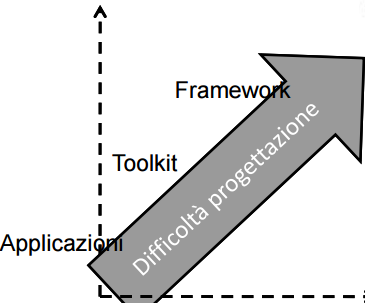
\includegraphics[width=0.3\columnwidth]{img1}
\begin{itemize}
	\item Applicazioni: riuso propriamente interno;
	\item Toolkit: librerie software che possono essere riusabili per progetti per fornire funzionalità generiche;
	\item Framework: insieme di classi che operano per costruire architetture riutilizzabili per sviluppare un dominio di applicazioni. Non sono design pattern in quanto questi ultimi sono più astratti, disegnano architetture più piccole e sono meno specializzati.
\end{itemize}

Ci sono dunque varie tipologie di pattern:
\begin{itemize}
	\item \textbf{Architetturali:} sono pattern di alto livello (MVC, Peer to peer, client-server);
	\item \textbf{Progettuali:} progettazione di dettaglio di componenti, definiscono micro architetture (Factory, Command, Proxy..)
	\item \textbf{Idiomi:} basso livello di astrazione, specifici del linguaggio di programmazione. Non sono propriamente dei design pattern infatti sono una soluzione specifica ad un linguaggio.
\end{itemize}
